\documentclass{beamer}
\usepackage{tikz}

\begin{document}

\begin{frame}
\frametitle{Age of Water under dye from all Rivers}

    \only<1-3>{\begin{tikzpicture}
        \node [](0,0)(start){ 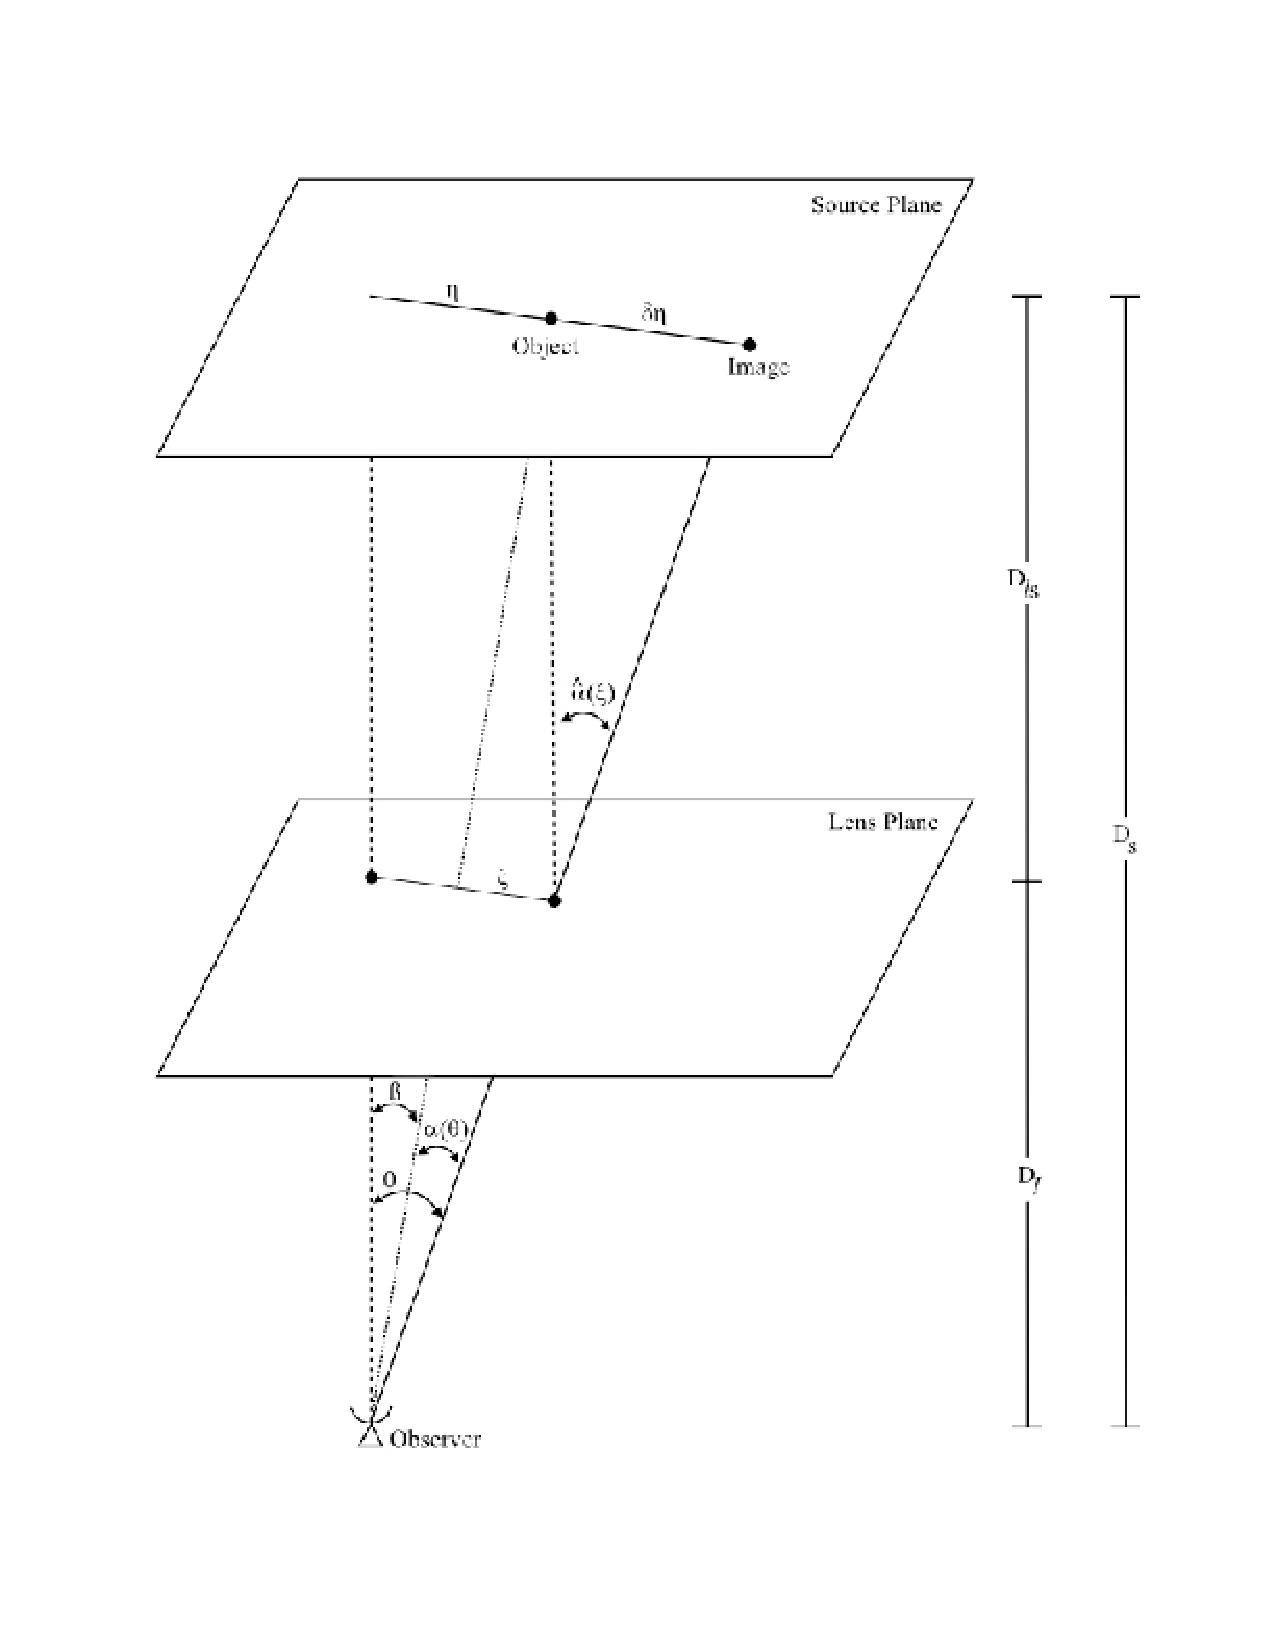
\includegraphics[height=4cm]{fig1}};
%       \draw [step=0.5cm,thin,dotted] (-5,-4) grid(5,4);
%       \node [circle]at (-4.5,0){0};
%       \node [circle,radius=0.9cm,fill=red!30,] at (-4.5,0)(a){};
        \onslide<2->{\draw [red,fill=red!30](-4.3,-0.2)circle(0.1cm);
        \draw [red,fill=red!30](-3.3,0)circle(0.1cm);
        \draw [red,fill=red!30](-2.5,-0.7)circle(0.1cm);
        \draw [red,fill=red!30](-4.,-0.8)circle(0.1cm);
        \draw [red,fill=red!30](-4.,-1.2)circle(0.1cm);
        \draw [red,fill=red!30](4.3,1.6)circle(0.1cm);
        \draw [red,fill=red!30](3.3,2.7)circle(0.1cm);
        \draw [red,fill=red!30](1.6,3.5)circle(0.1cm);
        \draw [red,fill=red!30](1.3,3.5)circle(0.1cm);}
        \node [rectangle,text width=4cm,red] at (5.5,3) (return) {$Q_2 = 169 A^{0.616}$     \linebreak Mason et. al. 1998};
        \onslide<3> \node [rectangle,text width=4cm,red] at (5,0) (return) {Smaller near the source     \linebreak Increases away from the source};
        \onslide<3> \draw [red](-3.3,-1.5) circle(0.7cm);%wolf bay small age
    \end{tikzpicture}}

        \only<4->{\begin{tikzpicture}
        \node [](0,0)(start){ 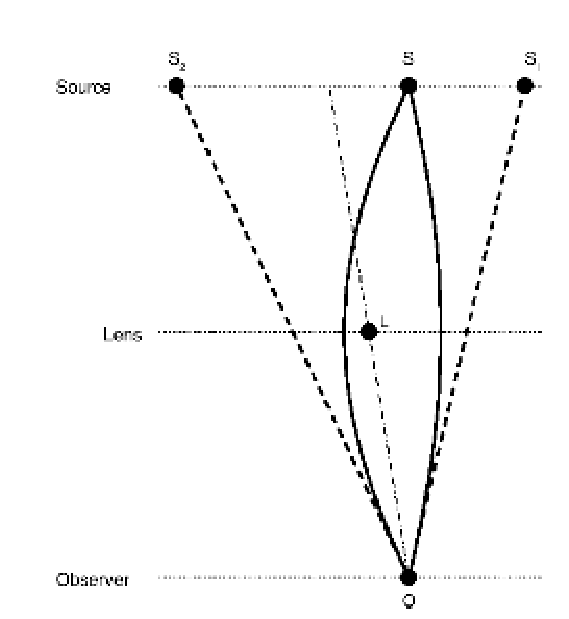
\includegraphics[height=4cm]{fig2}};
    \draw [step=0.5,dotted](-5,-4) grid (5,4);
    \end{tikzpicture}}
\end{frame}

\end{document}
